\chapter{Analyse et spécification des besoins}

\section*{Introduction}

Ce chapitre formalise ce que l'application doit faire et dans quelles
conditions. Il présente successivement les acteurs, les besoins
fonctionnels (regroupés en cas d'utilisation), puis les besoins non
fonctionnels (sécurité, performance, déploiement, maintenabilité).

\section{Description générale du projet}

\textbf{WebCyber} est une application web sécurisée de prise de notes
personnelle. Chaque utilisateur, après s'être inscrit puis authentifié,
peut créer, lire, modifier, archiver, supprimer (corbeille avec
restauration) et rechercher des notes textuelles qui lui sont propres.
Aucun utilisateur ne peut accéder aux notes d'un autre, même en
manipulant directement les URL ou les paramètres de requête.

L'application n'est donc pas une innovation fonctionnelle en elle-même
--- des solutions comparables (Google Keep, Microsoft OneNote, Apple
Notes) existent depuis longtemps. Le choix d'un domaine fonctionnel
familier est volontaire : il permet de \textbf{concentrer l'effort sur
la qualité de la conception, du déploiement et de la sécurité} plutôt
que sur la nouveauté de la fonctionnalité.

\section{Identification des acteurs}

Deux acteurs interagissent avec le système :

\begin{itemize}
  \item \textbf{Visiteur} : tout internaute non authentifié. Il peut
        accéder uniquement aux pages publiques (page d'accueil,
        formulaire de connexion, formulaire d'inscription).
  \item \textbf{Utilisateur authentifié} : un visiteur qui s'est
        connecté avec succès. Il accède à son espace personnel et y
        gère ses notes.
\end{itemize}

L'application n'embarque pas d'acteur \emph{Administrateur} : la
gestion des utilisateurs (création, suppression d'un compte) reste
manuelle, par accès direct à la base de données. Cette simplification
est cohérente avec le périmètre académique.

\section{Besoins fonctionnels}

\subsection{Liste des besoins}

\begin{longtable}{C{1.2cm} P{4.5cm} P{8cm}}
\toprule
\textbf{ID} & \textbf{Besoin} & \textbf{Description} \\
\midrule
\endhead

BF-01 & S'inscrire & Le visiteur saisit un nom d'utilisateur, un email et un mot de passe; le système crée un compte. \\
BF-02 & Se connecter & L'utilisateur saisit ses identifiants; le système vérifie le hachage et ouvre une session. \\
BF-03 & Se déconnecter & La session est détruite côté serveur; l'utilisateur revient à la page de connexion. \\
BF-04 & Créer une note & L'utilisateur saisit un titre et un contenu; la note est sauvegardée et associée à son compte. \\
BF-05 & Consulter ses notes & Affichage paginé des notes de l'utilisateur, par date de modification décroissante. \\
BF-06 & Voir une note en détail & Affichage du titre et du contenu complet d'une note. \\
BF-07 & Modifier une note & L'utilisateur édite le titre et/ou le contenu; la date de modification est mise à jour. \\
BF-08 & Archiver / désarchiver & La note est marquée \texttt{is\_archived}; elle disparaît de la liste principale et apparaît dans l'archive. \\
BF-09 & Mettre à la corbeille & La note est marquée \texttt{is\_trashed}; elle est cachée mais peut être restaurée. \\
BF-10 & Restaurer depuis la corbeille & Le drapeau \texttt{is\_trashed} est levé; la note revient dans la liste. \\
BF-11 & Supprimer définitivement & Suppression \texttt{DELETE} en base, irrécupérable. \\
BF-12 & Rechercher une note & Filtre par titre ou contenu; résultats limités au compte courant. \\
BF-13 & Isolation par utilisateur & Toute lecture, écriture ou suppression filtre par \texttt{user\_id} de la session courante. \\

\bottomrule
\end{longtable}

\subsection{Diagramme de cas d'utilisation}

La figure~\ref{fig:cas-utilisation} synthétise les cas d'utilisation et
leurs liens avec les acteurs. Les relations
\guillemotleft\,\emph{include}\,\guillemotright{} indiquent que les
opérations sur les notes nécessitent une authentification préalable
(BF-02).

\begin{figure}[H]
  \centering
  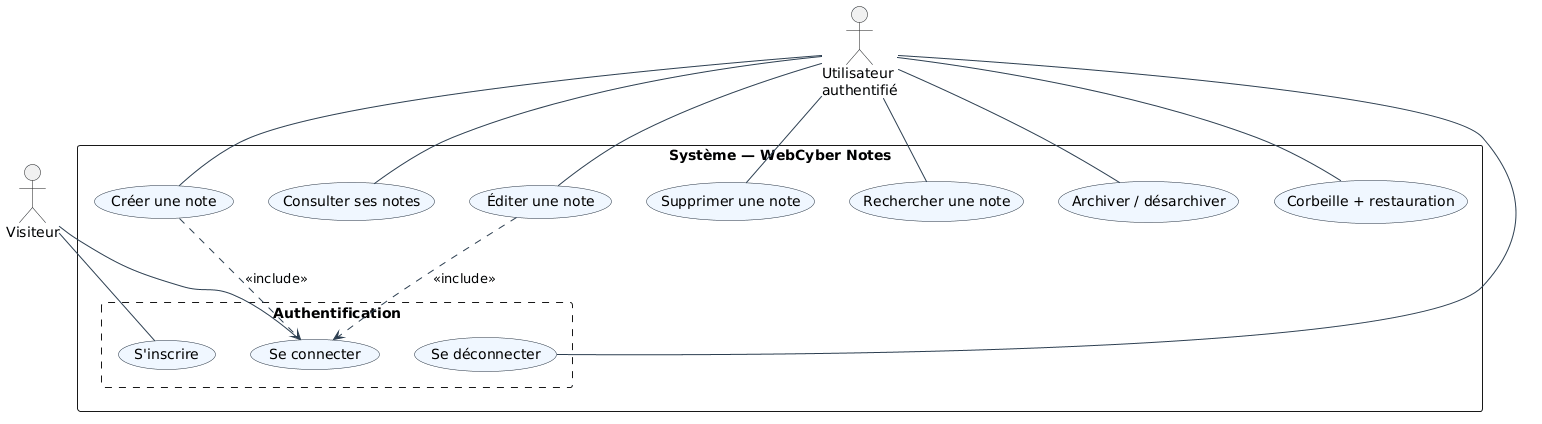
\includegraphics[width=\linewidth]{figures/img/fig04-cas-utilisation.png}
  \caption{Diagramme de cas d'utilisation de WebCyber.}
  \label{fig:cas-utilisation}
\end{figure}

\section{Besoins non fonctionnels}

Les besoins non fonctionnels traduisent les \emph{qualités attendues}
du système, indépendamment des fonctionnalités elles-mêmes.

\subsection{Sécurité}

\begin{itemize}
  \item \textbf{Confidentialité} : tout le trafic entre le client et le
        serveur doit être chiffré (HTTPS, TLS 1.2 ou 1.3).
  \item \textbf{Authentification forte} : les mots de passe ne sont
        jamais stockés en clair; un algorithme de hachage à coût
        configurable (PBKDF2-SHA256) est utilisé.
  \item \textbf{Protection contre les vulnérabilités OWASP Top 10} :
        en particulier les injections SQL, le XSS, le CSRF et les
        contournements de contrôle d'accès.
  \item \textbf{Isolation réseau} : seuls les ports strictement
        nécessaires (22, 80, 443) sont exposés au public.
  \item \textbf{Isolation des données} : un utilisateur ne peut en
        aucun cas accéder aux notes d'un autre.
\end{itemize}

\subsection{Disponibilité et performance}

\begin{itemize}
  \item \textbf{Disponibilité} : le projet ne vise pas la haute
        disponibilité; une instance EC2 unique suffit. Le redémarrage
        automatique des conteneurs (\texttt{restart: unless-stopped})
        couvre les pannes logicielles.
  \item \textbf{Performance} : la solution doit pouvoir servir une
        dizaine d'utilisateurs simultanés sur une instance \texttt{t2.micro}
        (1~vCPU, 1~Gio de RAM). Cela correspond largement aux besoins
        d'une démonstration ou d'un usage personnel.
\end{itemize}

\subsection{Déploiement et maintenabilité}

\begin{itemize}
  \item \textbf{Déploiement reproductible} : la solution doit pouvoir
        être redéployée \emph{from scratch} à partir du dépôt Git, en
        moins de trente minutes.
  \item \textbf{Conteneurisation complète} : aucun composant n'est
        installé directement sur l'hôte; tout passe par Docker
        Compose.
  \item \textbf{Documentation} : l'ensemble des choix d'architecture,
        de configuration et de sécurité est documenté de manière à
        permettre à un autre étudiant ou ingénieur de prendre la suite.
  \item \textbf{Renouvellement automatisé} des certificats TLS via
        Certbot (cron quotidien).
\end{itemize}

\subsection{Ergonomie}

\begin{itemize}
  \item Interface web responsive (mobile et desktop), basée sur
        \textbf{Tailwind CSS} pour un rendu moderne et cohérent.
  \item Navigation simple : barre latérale pour basculer entre la
        liste, l'archive et la corbeille; palette de commandes pour
        un accès rapide.
\end{itemize}

\subsection{Périmètre exclu}

Pour rester fidèle au cadre académique du PFE, certains éléments
classiques d'une production réelle sont \textbf{volontairement exclus} :

\begin{itemize}
  \item Orchestration Kubernetes ou multi-instance (\emph{auto-scaling});
  \item Pipeline CI/CD complet (GitHub Actions \(+\) déploiement
        automatique);
  \item \emph{Web Application Firewall}, services de protection AWS
        avancés (WAF, GuardDuty);
  \item Centralisation des journaux (CloudWatch, ELK);
  \item Monitoring applicatif (Prometheus, Grafana).
\end{itemize}

Ces éléments sont mentionnés dans la \textbf{conclusion générale}
comme perspectives d'évolution.

\section{Conclusion du chapitre}

L'analyse des besoins fait ressortir un système fonctionnellement
simple mais soumis à des exigences non fonctionnelles
\emph{nombreuses} (sécurité, déploiement reproductible, isolation,
HTTPS). Le chapitre suivant traduit ces exigences en une architecture
concrète : choix de l'infrastructure AWS, organisation des conteneurs
Docker, modèle de données, conception de la sécurité en profondeur.
